\documentclass[11pt, oneside]{article}   	% use "amsart" instead of "article" for AMSLaTeX format
\usepackage{geometry}                		% See geometry.pdf to learn the layout options. There are lots.
\geometry{letterpaper}                   		% ... or a4paper or a5paper or ... 
%\geometry{landscape}                		% Activate for for rotated page geometry
%\usepackage[parfill]{parskip}    		% Activate to begin paragraphs with an empty line rather than an indent
\usepackage{graphicx}				% Use pdf, png, jpg, or eps� with pdflatex; use eps in DVI mode
								% TeX will automatically convert eps --> pdf in pdflatex		
\usepackage{amssymb}
\usepackage{amsmath}
\usepackage{parskip}
\usepackage{color}

\title{Kepler (from Hartig Math 304)}
%\author{The Author}
%\section{}
% \subsection*{R code}
\date{}							% Activate to display a given date or no date

\graphicspath{{/Users/telliott_admin/Dropbox/Tex/png/}}

% \begin{center} 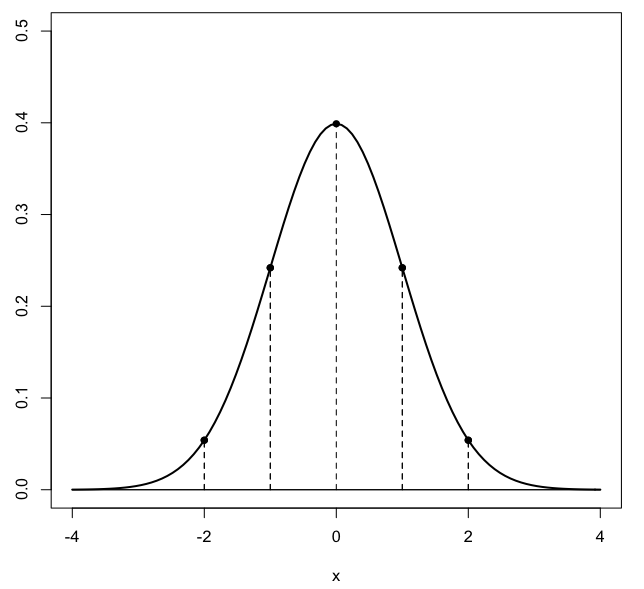
\includegraphics [scale=0.4] {gauss3.png} \end{center}

\begin{document}
\maketitle
\Large
\noindent

This is a derivation of Kepler's laws from the a class handout (Math 304) by Hartig.
\section{}
We start by defining $M$ as the mass of the sun and $m$ as the mass of a planet and $\mathbf{r}$ as the position vector from the sun to the planet.  Combining Newton's second law and the inverse square law of gravitation we have that 
\[ \mathbf{F} = m \mathbf{a} = -\frac{GMm}{r^2} \ \frac{\mathbf{r}}{r}  \]
\[ \mathbf{a} = -\frac{GM}{r^2} \ \frac{\mathbf{r}}{r}  \]
We take $\hat{\mathbf{u}}$ as a unit vector in the same direction as $\mathbf{r}$.  I will write $\hat{\mathbf{u}}$ without its hat as $\mathbf{u}$ so as not to confuse it with the derivative $\dot{\mathbf{u}}$.
\[ \mathbf{r} = r \mathbf{u} \]
\[ \mathbf{a} = -\frac{GM}{r^2} \ \mathbf{u}  \]
\section{}
Now, the velocity is the time-derivative of the position vector $\mathbf{r}$.
\[ \mathbf{v} = \frac{d\mathbf{r}}{dt} = \dot{\mathbf{r}} \]
and the acceleration is
\[ \mathbf{a} = \frac{d\mathbf{v}}{dt} = \ddot{\mathbf{r}} \]
because the force is toward the sun, the acceleration vector is parallel to the position vector, but with a change of sign.
\section{Feynman's dots}
We set up the angular momentum as
\[ \mathbf{L} = \mathbf{r} \times \mathbf{v} =  \mathbf{r} \times \dot{\mathbf{r}} \]
We compute the time-derivative
\[ \frac{d}{dt} (\mathbf{r} \times \dot{\mathbf{r}}) \]
by a standard vector application of the product rule which we've looked at elsewhere this is equal to 
\[ =  \dot{\mathbf{r}} \times \dot{\mathbf{r}} + \mathbf{r} \times \ddot{\mathbf{r}} \]
and this is equal to zero, since any vector's cross product with itself is zero, including a reversed version of itself, as is present in the second term.  This is just conservation of angular momentum
\[ \frac{d \mathbf{L}}{dt} = 0 \]
we will define a constant vector $\mathbf{c}$ rather than use $\mathbf{L}$ and say that
\[ \mathbf{c} = \mathbf{r} \times \dot{\mathbf{r}} \]
Since $\mathbf{c}$ is a constant, unchanging in both direction and magnitude, it defines a normal vector to the plane containing $\mathbf{r}$ and $\dot{\mathbf{r}}$.  We align $\mathbf{c}$ with the $z$-axis.  All the motion occurs in the $xy$-plane.
Note that 
\[ c = |\mathbf{c}| \]
\section{Equal area}
We consider the triangle formed by the position vector before and after a short period of time $\Delta t$, and the vector $\Delta \mathbf{r}$ connecting these two positions
\[ \Delta \mathbf{r} \approx \dot{\mathbf{r}} \Delta t \]
The little bit of area that is swept out during this time is 
\[ \Delta A \approx \frac{1}{2} \ |\mathbf{r} \times  \dot{\mathbf{r}} \Delta t | = \frac{1}{2} \ |\mathbf{c}| \Delta t \]
So we have that
\[ \frac{\Delta A}{\Delta t} \approx \frac{1}{2} \ c \]
and in the limit as $\Delta t \rightarrow 0$
\[ \frac{dA}{dt} = \frac{1}{2} \ c \]
\section{Manipulating $\mathbf{a} \times \mathbf{c}$}
The next step is to prove that
\[ \mathbf{a} \times \mathbf{c} = GM \dot{\mathbf{u}} \]
This takes a bit of work, so I'd like to put it off until the end.  We'll just assume it for now.
Take this equality and integrate it with respect to time, obtaining
\[ \int \mathbf{a} \times \mathbf{c} = \int GM \dot{\mathbf{u}} \]
\[ \dot{\mathbf{r}} \times \mathbf{c} = GM \mathbf{u} + \mathbf{d} \]
where $\mathbf{d}$ is a constant \emph{vector} of integration.
\section{Dot product}
We're almost there now.  Take the left-hand side from above and form the dot product
\[ \mathbf{r} \cdot (\dot{\mathbf{r}} \times \mathbf{c}) \]
Use another vector identity to switch it around
\[ = (\mathbf{r} \times \dot{\mathbf{r}}) \cdot \mathbf{c} \]
But this is just the definition of $\mathbf{c}$
\[ = \mathbf{c}  \cdot \mathbf{c} = c^2 \]
\section{Conic section}
So what we've shown is that
\[ c^2 = \mathbf{r} \cdot (GM \mathbf{u} + \mathbf{d} ) \]
\[ = r(GM + d \cos \theta) = rGM(1 + \frac{d}{GM} \cos \theta ) \]
Define $k = c^2/GM$ and $e = d/GM$.  Then
\[ k = r(1 +e\cos \theta) \]
This is the equation of a conic section.  In particular, if $ e < 1$, then
\[ r = \frac{k}{1 +e\cos \theta} \]
is the equation of an ellipse.  Here is an example with $k=1$ and $e=0.6$
\begin{center} 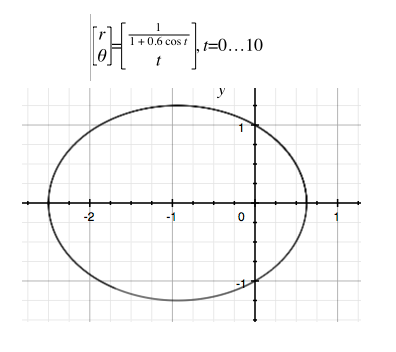
\includegraphics [scale=0.75] {ellipse_param.png} \end{center}
\section{Cleaning up}
To prove:
\[ \mathbf{a} \times \mathbf{c} = GM \dot{\mathbf{u}} \]
where $\hat{\mathbf{u}}$ is a unit vector and
\[ \mathbf{r} = r \hat{\mathbf{u}} \]
\[ \mathbf{r} = r \mathbf{u} \]
We recall that 
\[ \mathbf{c} = \mathbf{r} \times \mathbf{v} \]
so substitute into the left-hand side
\[ \mathbf{a} \times (\mathbf{r} \times \mathbf{v} ) \]
A standard result is that
\[ \mathbf{a} \times (\mathbf{r} \times \mathbf{v} ) = (  \mathbf{a} \cdot \mathbf{v}) \mathbf{r} - (  \mathbf{a} \cdot \mathbf{r}) \mathbf{v} \]
Recall that
\[ \mathbf{a} = - \frac{GM}{r^2} \mathbf{u} \]
\[ \mathbf{r} = r \mathbf{u} \]
\[ \mathbf{v} = \dot{\mathbf{r}} = \frac{d}{dt} \ r \mathbf{u} = \frac{dr}{dt} \mathbf{u} + r \dot{\mathbf{u}} \]
So let's work through it.  The first term is
\[ \mathbf{a} \cdot \mathbf{v} = - \frac{GM}{r^2} \mathbf{u} \cdot ( \frac{dr}{dt} \mathbf{u} + r \dot{\mathbf{u}}) \]
\[ = - \frac{GM}{r^2} \ \frac{dr}{dt} - \frac{GM}{r} \ \mathbf{u} \cdot \dot{\mathbf{u}} \]
and that all multiplies $\mathbf{r} = r \mathbf{u}$ 
\[ = - \frac{GM}{r} \ \frac{dr}{dt}  \mathbf{u}- GM \ (\mathbf{u} \cdot \dot{\mathbf{u}}) \mathbf{u} \]
The second term is
\[ \mathbf{a} \cdot \mathbf{r} = - \frac{GM}{r^2} \mathbf{u} \cdot r \mathbf{u} \]
\[ = - \frac{GM}{r} \]
which multiplies $\mathbf{v}$
\[ - \frac{GM}{r} (\frac{dr}{dt} \mathbf{u} + r \dot{\mathbf{u}}) \]
\[ = - \frac{GM}{r} \frac{dr}{dt} \mathbf{u} - GM \dot{\mathbf{u}}) \]
Now we subtract the second term from the first, so we have a cancellation and what is left is
\[  GM \dot{\mathbf{u}} - GM \ (\mathbf{u} \cdot \dot{\mathbf{u}}) \mathbf{u} \]
So somehow we need to show that 
\[ \mathbf{u} \cdot \dot{\mathbf{u}} = 0 \]

\end{document}  